\chapter{Materiales y métodos} % Main chapter title

\label{Chapter2}
\definecolor{mygreen}{rgb}{0,0.6,0}
\definecolor{mygray}{rgb}{0.5,0.5,0.5}
\definecolor{mymauve}{rgb}{0.58,0,0.82}

\lstset{ %
  backgroundcolor=\color{white},   % choose the background color; you must add \usepackage{color} or \usepackage{xcolor}
  basicstyle=\footnotesize,        % the size of the fonts that are used for the code
  breakatwhitespace=false,         % sets if automatic breaks should only happen at whitespace
  breaklines=true,                 % sets automatic line breaking
  captionpos=b,                    % sets the caption-position to bottom
  commentstyle=\color{mygreen},    % comment style
  deletekeywords={...},            % if you want to delete keywords from the given language
  %escapeinside={\%*}{*)},          % if you want to add LaTeX within your code
  %extendedchars=true,              % lets you use non-ASCII characters; for 8-bits encodings only, does not work with UTF-8
  %frame=single,	                   % adds a frame around the code
  keepspaces=true,                 % keeps spaces in text, useful for keeping indentation of code (possibly needs columns=flexible)
  keywordstyle=\color{blue},       % keyword style
  language=[ANSI]C,					% the language of the code
  %otherkeywords={*,...},           % if you want to add more keywords to the set
  numbers=left,                    % where to put the line-numbers; possible values are (none, left, right)
  numbersep=5pt,                   % how far the line-numbers are from the code
  numberstyle=\tiny\color{mygray}, % the style that is used for the line-numbers
  rulecolor=\color{black},         % if not set, the frame-color may be changed on line-breaks within not-black text (e.g. comments (green here))
  showspaces=false,                % show spaces everywhere adding particular underscores; it overrides 'showstringspaces'
  showstringspaces=false,          % underline spaces within strings only
  showtabs=false,                  % show tabs within strings adding particular underscores
  stepnumber=1,                    % the step between two line-numbers. If it's 1, each line will be numbered
  stringstyle=\color{mymauve},     % string literal style
  tabsize=2,	                   % sets default tabsize to 2 spaces
  title=\lstname,                   % show the filename of files included with \lstinputlisting; also try caption instead of title
  morecomment=[s]{/*}{*/}%
}



%----------------------------------------------------------------------------------------
%	SECTION 1
% Aquí se mencionan los componentes que se utilizaron y la metodología empleada.
% Luego pueden ir las plaquetas que se diseñaron para el prototipo, esquemáticos,
% diagrama de flujo, dibujos en 3D, etc.
%----------------------------------------------------------------------------------------


El presente trabajo formó parte de un proyecto más grande. Consistió en la realización de dos sistemas, CFAR y configurador, los cuales eran subsistemas de un Procesador Monoradar.

La partición del diseño se realizó teniendo en cuenta las distintas funciones a realizar. Para este proyecto, el sistema CFAR se diseñó para generar el umbral adaptativo propio de la técnica mencionada. Luego, teniendo en cuenta que el clutter se concentra en general en las inmediaciones del radar y que se podría tener mejor desempeño en el filtrado admitiendo distintos factores de escala CFAR en distintas zonas de la cobertura, se diseño el sistema configurador para poder sectorizar la cobertura en un determinado número de sectores independientes. Además, se incorporó al configurador ciertas funciones para realizar un ajuste automático en el valor de escala CFAR para cumplir una determinada cantidad de presencia requerida por el usuario.

Para la realización del presente trabajo se utilizó:
\begin{itemize}
\item Placa ADC-SoC de TerasIC.
\item Software Quartus Prime.
\item Software ModelSim.
\item Software VHDL Style Guide.
\item Sistema de control de versiones GIT.
\item Repositorio remoto en GitHub.
\item Procesador monoradar preexistente.
\item Simulador de radar.

\end{itemize}

En las secciones siguientes se menciona la utilización de las mismas.

\section{Placa ADC-SoC de TerasIC}
Se utilizó una placa tipo SoC-FPGA de la firma TeraSiC. Esta placa posee un circuito de conversión analógica a digital que utiliza conectores SMA como interfaz de entrada y proporciona dos canales de conversión, cada uno de 14-bits de resolución y una frecuencia de muestreo de hasta 150 MSPS (Megasamples per Second).

\begin{figure}
\centering
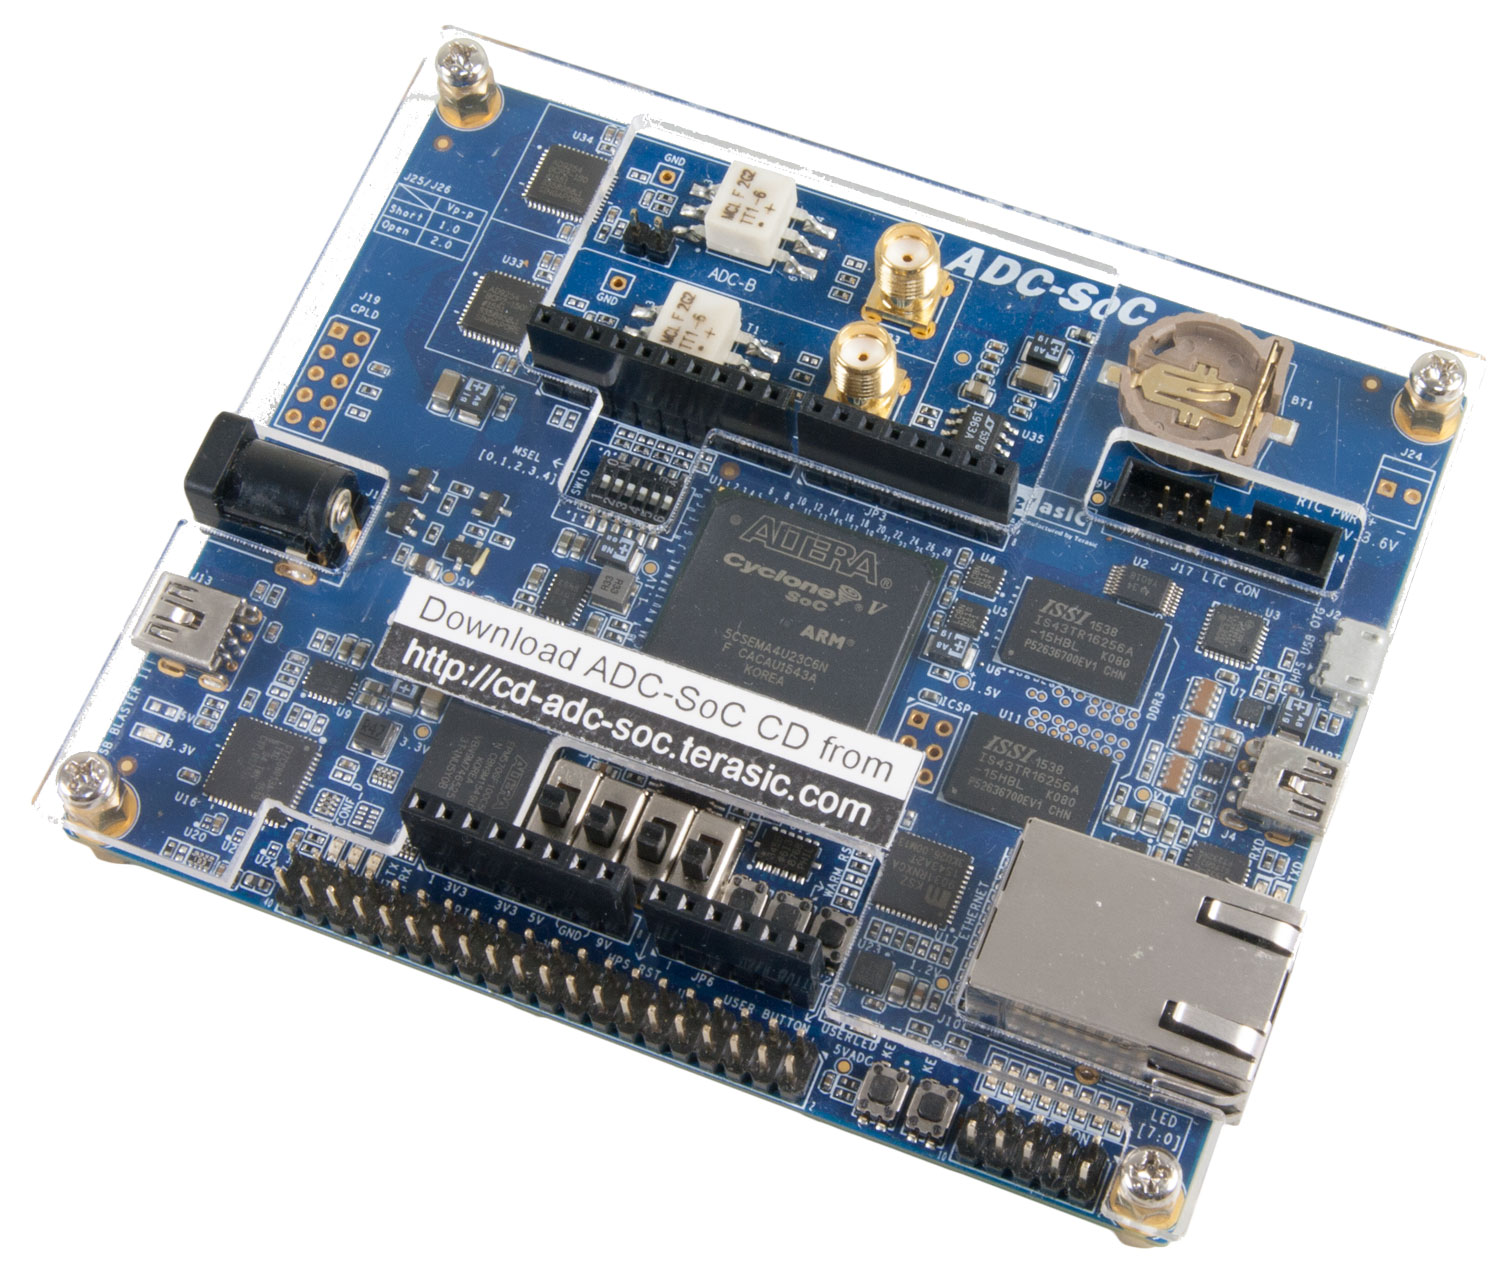
\includegraphics[scale=0.15]{./Figures/ADC-SoC.jpg}
\caption{Placa ADC-SoC de TerasIC}
\end{figure}

El siguiente hardware se proporciona en la placa:

\begin{itemize}
\item 	FPGA
	\begin{itemize}
	\item Dispositivo Altera Cyclone V.
	\item Dispositivo de configuración en serie.
	\item USB-Blaster II integrado para programación; Modo JTAG
	\item 2 pulsadores
	\item 4 interruptores deslizantes
	\item 8 LED de usuario verdes
	\item Tres fuentes de reloj de 50 MHz del generador de reloj
	\item Un cabezal de expansión de 40 pines
	\item Un encabezado de expansión Arduino (compatibilidad con Arduino Uno R3) donde se puede conectar los 'shields' Arduino.
	\item Un encabezado de expansión de entrada analógica de 10 pines (compartido con la entrada analógica Arduino).
	\item Convertidor A / D, interfaz SPI de 4 pines con FPGA
	\item  Dos convertidores AD de 14 bits con 150 MSPS (megamuestras por segundo)
	\end{itemize}
	
	
\item HPS (Hard Processor System)
	\begin{itemize}
	\item Procesador ARM Cortex-A9 de doble núcleo de 925 MHz
	\item 1GB DDR3 SDRAM (bus de datos de 32 bits)
	\item 1 Gigabit Ethernet PHY con conector RJ45
	\item Puerto USB OTG, conector USB Micro-AB
	\item Toma de tarjeta micro SD
	\item Acelerómetro (interfaz I2C + interrupción)
	\item UART a USB, conector USB Mini-B
	\item Botón de reinicio en caliente y botón de reinicio en frío
	\item Un botón de usuario y un LED de usuario
	\item Cabecera de expansión LTC 2x7
	\item RTC integrado (reloj en tiempo real)
	\end{itemize}
\end{itemize}


\begin{figure}
\centering
\includegraphics[scale=0.25]{./Figures/ADC-SoC_blockdiagram.jpg}
\caption{Diagrama en bloques de la placa ADC-SoC de TerasIC}
\end{figure}


En el chip Cyclone V de Altera (propiedad de Intel) se integra una FPGA y un HPS unidos por un puente HPS. Por defecto, la tarjeta micro SD tiene instalado el SO “​Linux Yocto Poky 8.0​”, el cual permite correr programas compilados en lenguaje C/C++ entre otros.
 
 
\section{Quartus Prime}
Como herramienta de compilación se utilizó \textit{Quartus Prime}, software producido por Altera para el análisis y la síntesis de diseños realizados en HDL. Permite compilar diseños, realizar análisis temporales, examinar diagramas RTL y configurar el dispositivo de destino con el programador.

\textit{Quartus} proporciona herramientas para trabajar en diferentes fases del diseño en FPGA como la creación del diseño, el agregado de restricciones, la compilación, el análisis de tiempos y la configuración de la FPGA con un programador. Se describen las características de \textit{Quartus} a continuación:

\begin{itemize}
\item
Creación del diseño: Es posible diseñar en nivel RTL con lenguajes VHDL, Verilog o SystemVerilog. Además posee una herramienta llamada \textit{Platform Designer} que crea automáticamente la lógica de interconexión a partir de la conectividad de alto nivel que se especifique. La automatización de interconexión elimina la laboriosa tarea de especificar conexiones HDL a nivel del sistema. De esta manera se pueden  especificar los requisitos de la interfaz e integrar componentes de IP dentro de una representación gráfica del sistema. En el presente proyectó se utilizó \textit{Platform Designer} (Diseñador de plataformas) para configurar el puente HPS.
\item
Permite el agregado de restricciones al diseño con herramientas denominadas \textit{assigment editor} (Editor de asignaciones) y \textit{pin planner} (Planificador de pines).
\item
Permite compilar el diseño, compuesto por las siguientes etapas:
\begin{itemize}
	\item
	Análisis y Síntesis
	Se evalúa el código para detectar la correcta escritura del mismo y se verifica que el mismo sea sintetizable, es decir que pueda ser implementado con lógica.
	\item
	\textit{Fitter} (Consiste en la colocación y Ruteo, \textit{Place \& Route}): Se asignan recursos específicos de la FPGA para cumplir con el diseño. En etapa etapa además la herramienta utiliza la información sobre las restricciones de tiempo evaluar qué celdas utilizar (en términos de propagación de señales). Por otro lado, luego de la colocación, se emplean técnicas de optimización en la asignación de recursos.
	\item
	Generación de archivos de programación: Se generan los archivos necesarios para programar la FPGA.
	\item
	 Análisis de tiempo: Verifica mediante la herramienta \textit{Timing Analyzer} que se cumplan con las restricciones de tiempo especificadas en el diseño. Por ejemplo los referidos a la generación de señales de reloj internas, derivadas de fuentes de señales de reloj externas.
	\end{itemize}
	
\item 
Posee una herramienta llamada \textit{Signal Tab Logic Analyzer} que permite realizar un debug mientras el sistema se ejecuta en la FPGA.

\end{itemize}

\subsubsection{Visores de netlist}
\label{seccion: Visores de netlist}
A medida que los diseños de FPGA crecen en tamaño y complejidad, la capacidad de analizar, depurar, optimizar y restringir el diseño es fundamental. \textit{Quartus} posee visores llamados \textit{RTL Viewer}, \textit{State Machine Viewer} y \textit{Technology Map Viewer} (visores de nivel de transferencia de registros, de máquina de estados y de mapa tecnológico, respectivamente). Cada uno permite ver representaciones esquemáticas de la estructura interna del diseño. Cada visor muestra una vista única del \textit{netlist} (lista de redes) que se producen en diferentes etapas de la compilación, como se ilustra en la figura \ref{fig:netlist_viewers}. Se describen a continuación:

\begin{figure}
\centering
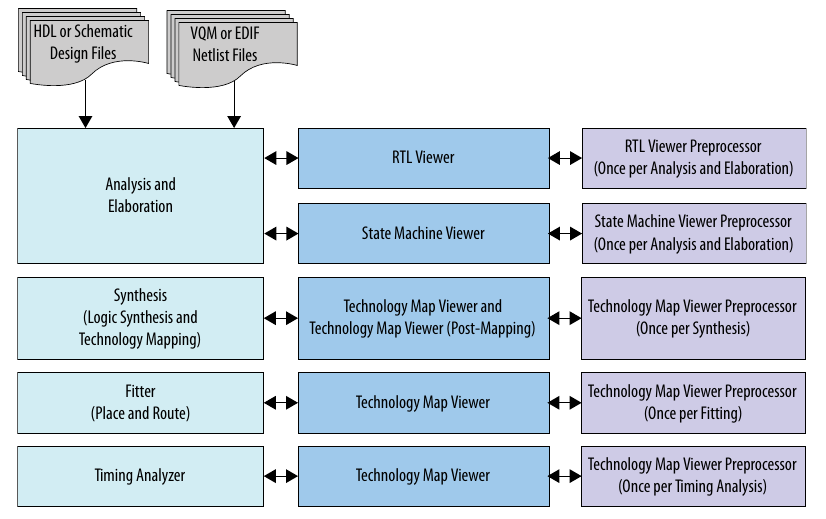
\includegraphics[scale=0.6]{./Figures/netlist_viewers.png}
\caption{Ubicación de los visores de netlist en el flujo de diseño de Quartus}
\label{fig:netlist_viewers}
\end{figure}

\begin{itemize}
\item
\textit{RTL Viewer}:
Permite ver un esquema de la lista de conexiones de diseño después de la etapa de Análisis y elaboración, y de la extracción de la lista de conexiones, pero antes de la síntesis y las optimizaciones de ajuste. Esta vista no es la estructura final del diseño, porque no se incluyen todas las optimizaciones; en cambio, es la vista más cercana posible al diseño original. Si el diseño utiliza síntesis integrada, esta vista muestra cómo \textit{Quartus} interpreta los archivos de diseño.

\item
\textit{State Machine Viewer}
Proporciona una vista de alto nivel de las máquinas de estados finitos en el diseño y muestra la estructura interna de las máquinas de estados en el diseño, incluida una vista más detallada de la entrada y salida de los nodos de estado individuales. También muestra las transiciones de los nodos en formato de tabla.

\item
\textit{Technology Map Viewer}
Permite ver un esquema de bajo nivel específico de la tecnología de la lista de redes de diseño después del ajuste o después de Análisis y síntesis. Se puede acceder a la vista del esquema \textit{post-fitting} (posterior al ajuste) o \textit{post-mapping} (posterior al mapeo), independientemente de la herramienta de síntesis que se utilice.

\end{itemize}


\subsection{ModelSim}

La simulación es un paso crítico en el diseño para FPGA. Permite al diseñador estimular su diseño y ver cómo el código que escribió reacciona al estímulo. Una gran simulación contendrá todos los estados posibles del diseño para garantizar que todos los escenarios de entrada se manejen de manera adecuada. Este ejercicio permite descubrir si en alguna parte del diseño, por ejemplo en procesos combinacionales,  no se contempló todos casos posibles y en caso de descubrir un comportamiento no esperado se procede a corregirlo.

Para este proyecto se utilizó ModelSim, un entorno de simulación creado por Mentor Graphics. ModelSim Está diseñado para trabajar con Verilog y VHDL. Además cuenta con un debugger, el cual se puede emplear, por ejemplo, para descubrir comportamientos más difíciles de dilucidar que no son determinados a simple vista.

\subsection{Sentencias VHDL tipo \textit{report} y \textit{assert}}
Las sentencias de \textit{report} y \textit{assert} son sentencias de VHDL que se utilizaron para verificar la correcta ejecución de los procesos. La sentencias tipo \textit{report} arroja un mensaje en la consola de acuerdo a nivel de severidad, cuando el programa pasa por dicha sentencia, se puede imprimir un mensaje en la consola y agregar el valor que tiene una señal o variable determinada. Las sentencias tipo \textit{assert} evalúan el valor de una variable o señal en función de una condición y reportan el resultado en la consola de acuerdo al nivel de severidad.

La sintaxis básica de las declaraciones tipo \textit{report} en VHDL es:


\begin{lstlisting}[caption= "Sintaxis tipo \textit{report}"]
	report <message_string> [severity <severity_level>];
\end{lstlisting}


\textit{Message string} es la cadena del mensaje. \textit{Severity level} es el nivel de gravedad del reporte. Los valores posibles de niveles de gravedad son: nota, advertencia, error, falla.

Las declaraciones tipo \textit{report} son declaraciones secuenciales. Esto significa que solo pueden estar en regiones secuenciales, como dentro de las declaraciones que forman parte de un \textit{process}. No pueden estar solos en una arquitectura.

Por otro lado, las declaraciones tipo \textit{assert} pueden ser secuenciales o concurrentes. Es decir, se pueden escribir en un proceso o en una arquitectura. Existen varias formas de escribir una declaración de este tipo, donde la condición es de tipo booleano:


\begin{lstlisting}[caption= "Sintaxis tipo \textit{assert}"]
	assert <condition>;
	assert <condition> severity <severity_level>;
	assert <condition> report <message_string>;
	assert <condition> report <message_string> severity <severity_level>;
\end{lstlisting}

\subsection{Buenas prácticas en la codificación VHDL}

\subsubsection{Guía de estilo de codificación VHDL}
Como se mencionó anteriormente, los sistemas desarrollados se diseñaron como subsistemas de un EDDR. Al ser el EDDR un proyecto más grande, involucró el trabajo de tres desarolladores y para unificar criterios de escritura del código VHDL se utilizó una guía de estilo de codificación.

Durante el proceso de revisión de código puede suceder que un problema real sea enmascarado por un problema de estilo de codificación. Dependiendo del proceso, los problemas de estilo pueden tardar mucho en resolverse. Por ejemplo, una serie de pasos a ejecutar podría ser:

\begin{itemize}
\item Crear una prueba.
\item Encontrar el problema.
\item Corregir el problema.
\item Verificar solución del problema.

\end{itemize}

Mantener un estilo de codificación permite por un lado, disminuir la probabilidad de errores y mejorar la lectura para uno mismo y para otros, especialmente durante el desarrollo del código en donde se comparte el trabajo con otros desarrolladores. Por el otro, dedicar menos tiempo a cuestiones de estilo deja más tiempo para analizar la estructura del código.

La eliminación de problemas de estilo reduce la cantidad de tiempo que se tarda en realizar las revisiones de código. Esto da como resultado una base de código de mayor calidad. Por ello, en este trabajó se utilizó un software, desarrollado por Jeremiah C Leary, denominado VSG (del acrónimo VHDL Style Guide).

Las características más destacadas de este programa son:
\begin{itemize}
\item
Definición explícita de los estándares de codificación VHDL.
\item
Configurable. Esto permite la actualización del código a los estándares actuales.
\item
Definición de un estilo del código y aplicación en partes o en toda la base del código.
\end{itemize}
El programa analiza el archivo cargado evaluando si el código cumple con todas las reglas de estilo, por ejemplo que todos los process tengan una etiqueta o que haya una correcta identación en las diferentes secciones del código. En caso de no hacerlo, VSG informará la regla que se viola y el número de línea o grupo de líneas donde ocurrió la violación. También da una sugerencia sobre cómo corregir la infracción.

La utilización de esta herramienta consistió en analizar cada entidad de diseño con el software y luego, realizar las correcciones pertinentes según el reporte de reglas incumplidas en cada archivo.

Para cuestiones que no están al alcance del software VSG se utilizó una convención para nombrar a puertos y señales

\subsubsection{Reglas de codificación}
Se adoptó las reglas de codificación propuestas por el departamento de sistemas informáticos de la Universidad Tecnológica de Tampere con el objetivo de aumentar la legibilidad para fines de revisión y evitar formas de codificación dañinas o poco prácticas. Se mencionan las más importantes a continuación:

\begin{itemize}
\item Usar solamente puertos tipo IN (de entrada) y tipo OUT (de salida).
\item Usar salidas registradas.
\item Realizar un \textit{test bench} por cada entidad de diseño.
\item Usar el flanco ascendente como flanco activo.
\item Hacer que los procesos síncronos sean sensibles sólo al \textit{clock} y \textit{reset}.
\item Hacer que los procesos combinacionales o asíncronos sean sensibles a todas las señales leídas en su interior.
\item Definir vectores en sentido descendente, tipo \textit{downto}.
\item Evitar números mágicos. Es decir, números que sólo el diseñador entiende de donde se originan. Emplear uso de constantes en su lugar.
\item Completar con todos los casos posibles las declaraciones secuenciales (por ejemplo \textit{if}, \textit{case}, etc).
\end{itemize}

\subsubsection{Otras convenciones}
Adicionalmente a lo mencionado anteriormente en ésta sección, se adoptaron convenciones propuestas por el equipo de desarrolladores del EDDR para nombres. Se mencionan a continuación:
\begin{itemize}
\item \textit{i\_ nombre} para puertos de entrada.

\item \textit{o\_ nombre} para puertos de salida.

\item \textit{nombre\_ s} para señales (cabe recordar que son de uso interno de la entidad).

\item \textit{nombre\_ v} para variables (función similar a señales).

\item \textit{i\_ nombre\_ numeración} para instancias.

\item \textit{nombre\_ g} para genéricos.

\end{itemize}


\section{Buenas prácticas en el diseño digital}

Al diseñar con código HDL, se debe comprender cómo una herramienta de síntesis interpreta las diferentes técnicas de diseño HDL y qué resultados esperar. Las diferentes técnicas de diseño pueden afectar la utilización de la lógica y el desempeño en cuanto al tiempo, así como la confiabilidad del diseño. Las buenas prácticas de diseño sincrónico están hechas para evitar la dependencia de los retrasos de propagación en un dispositivo, lo que puede provocar análisis de tiempos incompletos y posibles fallos. Se adoptó para este proyecto, las prácticas de diseño recomendadas por Altera (empresa fabricante del chip utilizado).


Se utilizó un diseño síncrono. En un diseño de este tipo, una señal de reloj controla la actividad de todas las entradas y salidas. El diseño se comporta de manera predecible y confiable para todas las condiciones de proceso, voltaje y temperatura (PVT) siempre que se asegure de que se cumplen todos los requisitos de temporización de los registros. Además es posible migrar fácilmente diseños síncronos a diferentes familias de dispositivos o grados de velocidad.


Se utilizó en todos los componentes los flancos activos del reloj parar disparar eventos. En cada flanco activo del reloj (que normalmente es el flanco ascendente), las entradas de datos de los registros se muestrean y se transfieren a las salidas. Siguiendo un flanco de reloj activo, las salidas de la lógica combinacional que alimentan las entradas de datos de los registros cambian de valor. Este cambio desencadena un período de inestabilidad debido a los retrasos de propagación a través de la lógica, ya que las señales pasan por varias transiciones y finalmente se establecen en nuevos valores. Los cambios que ocurren en las entradas de datos de los registros no afectan los valores de sus salidas hasta después del siguiente flanco de reloj activo. Debido a que el circuito interno de los registros aísla las salidas de datos de las entradas, la inestabilidad en la lógica combinacional no afecta el funcionamiento del diseño siempre que cumpla con los siguientes requisitos de tiempo:

\begin{itemize}
\item
Antes de un flanco de reloj activo, la entrada de datos haya sido estable durante al menos el tiempo de configuración del registro (\textit{setup time}).
  
\item
Después de un flanco de reloj activo, la entrada de datos permanezca estable durante al menos el tiempo de retención del registro (\textit{hold time}).
  
\end{itemize}

Al especificar todas las frecuencias de reloj y otros requisitos de tiempo, se puede utilizar la herramienta \textit{Timing Analyzer} descrita anteriormente para obtener un informe de los requisitos de hardware reales para los tiempos de configuración y tiempos de retención de cada pin del diseño. Al cumplir con estos requisitos de pines externos y seguir las técnicas de diseño sincrónico, se asegura el cumplimiento de los tiempos de configuración y retención para todos los registros del dispositivo utilizado.

Para cumplir con los requisitos de configuración y tiempo de espera en todos los pines de entrada, cualquier entrada a la lógica combinacional que alimenta un registro debe tener una relación sincrónica con el reloj del registro. Si las señales son asíncronas, se puede registrar las señales en las entradas del dispositivo para ayudar a prevenir una violación de los tiempos de retención y de configuración requeridos. Cuando no se cumplen estos requisitos, la salida de un registro puede oscilar la salida o establecer la salida en un nivel de voltaje intermedio entre los niveles alto y bajo llamado estado \textit{metaestable}. En este estado inestable, pequeñas perturbaciones, como el ruido en los rieles de alimentación, pueden hacer que el registro asuma el nivel de voltaje alto o bajo, dando como resultado un estado válido impredecible. Pueden producirse varios efectos indeseables, incluidos mayores retrasos de propagación y estados de salida incorrectos. En algunos casos, la salida puede incluso oscilar entre los dos estados válidos durante un período de tiempo relativamente largo.

\subsubsection{Lógica combinacional}

Las estructuras lógicas combinacionales constan de funciones lógicas que dependen únicamente del estado actual de las entradas. En las FPGA de Altera, estas funciones se implementan en LUT's con elementos lógicos o módulos lógicos adaptativos (ALM).

Los bucles combinacionales se encuentran entre las causas más comunes de inestabilidad y falta de fiabilidad en los diseños digitales. Los bucles combinacionales generalmente violan los principios de diseño síncrono al establecer un bucle de retroalimentación directa que no contiene registros. En un diseño síncrono, los circuitos de retroalimentación deben incluir registros. Por ejemplo, un bucle combinacional ocurre cuando el lado izquierdo de una expresión aritmética también aparece en el lado derecho en el código HDL. Un bucle combinacional también ocurre cuando retroalimenta la salida de un registro a un pin asincrónico del mismo registro a través de la lógica combinacional. En la sección siguiente se describirá una metodología que previene este tipo de bucles.

Otras recomendaciones tenidas en cuenta en el proceso de diseño fue la de evitar \textit{latches} inintencionales. Un \textit{latch} es un circuito pequeño con retroalimentación combinatoria que mantiene un valor hasta que se asigna un nuevo valor. Es común que los errores en el código HDL provoquen una inferencia de \textit{latch} no intencionada. A diferencia de otras tecnologías, un \textit{latch} en la arquitectura FPGA no es significativamente más pequeño que un registro. La arquitectura no está optimizada para la implementación de \textit{latches} y estos generalmente tienen un rendimiento de temporización más lento en comparación con los circuitos registrados equivalentes.



\subsection{Metodología estructurada}
\label{metodologia_estructurada}
Para algunos componentes se empleó la metodología propuesta por Jiri Gaisler de \textit{Gaisler Research}. Se realizó de esa manera para asegurar la síntesis en aquellos componentes donde había más procesamiento del tipo combinacional.

De acuerdo a autor, en el diseño  tradicional se presentan a menudo muchas declaraciones concurrentes, muchas señales y procesos de pocas líneas, entre otros. Esto puede ocasionar problemas, por ejemplo, en cuanto a:

\begin{itemize}
\item
Tiempo de ejecución (dependiendo del número de procesos).

\item 
Dificultad para entender el flujo de datos y/o el algoritmo.

\item
No distinguir entre señales del tipo secuencial y combinacional y señales relacionadas.

\end{itemize}

Para que el código sea fácil de entender y mantener, apto para rápida simulación, sintetizable y con menor posibilidad de discrepancias entre simulación y síntesis, el autor propone una abstracción de la lógica digital usando dos partes, como se ilustra en la figura \ref{2_process_scheme} , una secuencial y otra combinacional.

\begin{figure}
\centering
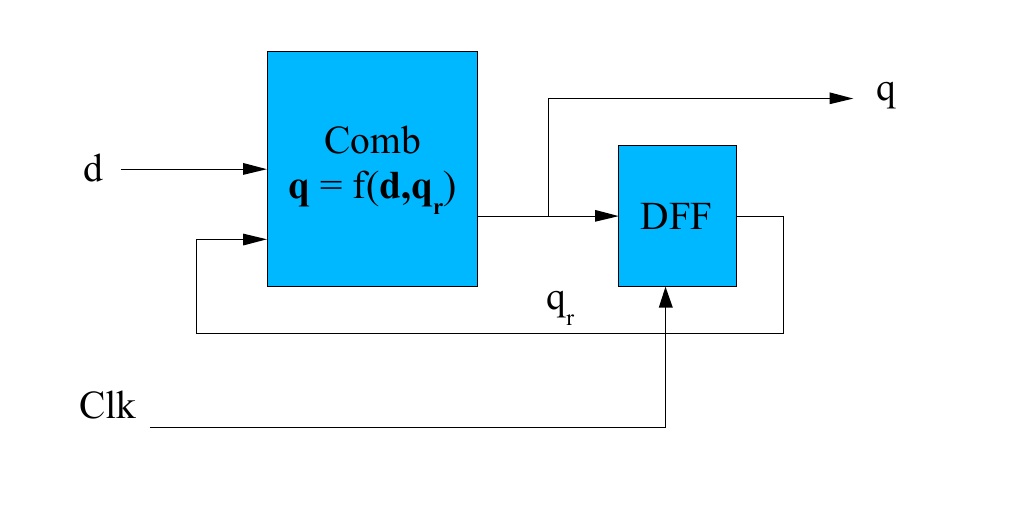
\includegraphics[scale=0.5]{./Figures/2_process_scheme.png}
\caption{Diseño sincrónico abstraído en dos partes, combinacional (izquierda) y secuencial (derecha)}
\label{2_process_scheme}
\end{figure}

Se implementó ésta metodología en VHDL de la siguiente manera:

\begin{itemize}
\item
La arquitectura albergó dos procesos: uno secuencial y otro combinacional.
\item
Se declaró dos señales locales, para entrada y salida del registro.
\item
Todo el algoritmo se volcó en el proceso combinacional.
\item
La lista de sensibilidad del proceso combinacional se realizó de modo que sea sensible a todos los puertos de entrada.
\item
La lista de sensibilidad del proceso secuencial se realizó de modo que sea sensible sólo a puerto de reloj.
\end{itemize}




\section{Diseño detallado}

\subsection{Partición Software $\&$ Hardware}
Uno de los primeros pasos para la realización de un diseño digital es la partición entre software y hardware. Es decir, decidir qué parte del diseñó se procesará con software y qué parte con hardware. A continuación se describe el detalle de la partición software/hardware para el CFAR y configurador:

\begin{itemize}
\item CFAR
	\begin{itemize}
	\item Componente de Firmware FPGA:
		\begin{itemize}
		\item Sistema CFAR de 64 celdas de referencia y 5 celdas de guarda.
		\item Posibilidad de alternar entre algoritmos CFAR.
		\item Celdas de 14-bit de resolución.
		\item Uso de coeficiente multiplicador de 16-bit.
		\end{itemize}
		
	\item Componente de Software HPS:
		\begin{itemize}
		\item Lectura de cuenta de targets (salida del CFAR).
		\end{itemize}
	
	\end{itemize}

\item Configurador
	\begin{itemize}
	\item Componente de Firmware FPGA:
		\begin{itemize}
		\item 32 sectores reducidos que abarquen cada uno una porción de la cobertura.
		\item 1 sector fijo que abarque toda la cobertura. 
		\item Posibilidad de alternar entre sector fijo y sectores reducidos.
		\item Control del tipo de video a utilizar (normal o integrado).
		\end{itemize}
	
	\item Componente de Software HPS:
		\begin{itemize}
		\item Control de coeficiente multiplicador.
		\item Control de coeficiente de ventana.
		\item Control del algoritmo.
		\item Control de tipo de filtrado.
		\item Control del modo de operación.
		\item Control del submodo de operación.
		\item Lectura de cuenta de multiplicador, algoritmo y ventana.
		\end{itemize}
		
	\end{itemize}
\end{itemize}

\subsection{Acciones del CFAR}
Se implementó la siguiente jerarquía de entidades de diseño para el CFAR:

\begin{itemize}
\item CFAR
	\begin{itemize}
	\item Celdas de referencia
		\begin{itemize}
		\item FFD
		\end{itemize}
	\item Celdas de guarda
		\begin{itemize}
		\item FFD
		\end{itemize}
	\item Celda test
	\item Comparador
	\end{itemize}

\item Contador CFAR

\end{itemize}



\begin{figure}
\centering
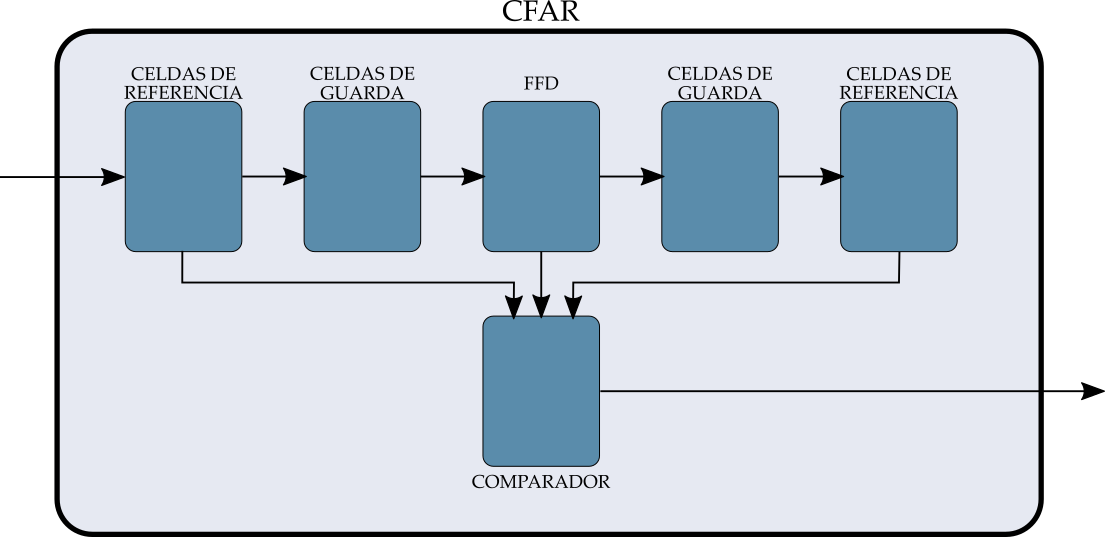
\includegraphics[scale=0.45]{./Figures/cfar_diag_bloques.png}
\caption{Relación entre componentes del CFAR}
\label{diagrama_cfar}
\end{figure}

La relación entre entidades de diseño del CFAR y el flujo de información entre estos se ilustra en la figura \ref{diagrama_cfar}.

Cada componente fue diseñado para realizar las acciones que se describen a continuación.

\subsubsection{FFD}
\begin{itemize}
\item Debe funcionar como un registro de 14-bit de carga y salida paralela.
\item Debe transferir cada bit del vector en un flanco ascendente del reloj.
\item Debe resetearse de forma asincrónica.
\item Debe permitir habilitación o deshabilitación.
\end{itemize}



\subsubsection{Celdas de guarda}
\begin{itemize}
\item Debe comportarse como un registro de desplazamiento de 5 celdas.
\item Debe transferir el dato de video en cada flanco ascendente del reloj.
\item Debe resetearse de forma asincrónica.
\item Debe permitir habilitación o deshabilitación.
\end{itemize}


\subsubsection{Celdas de referencia}
\begin{itemize}
\item Debe comportarse como un registro de desplazamiento de 64 celdas.
\item Debe transferir el dato de video en cada flanco ascendente del reloj.
\item Debe resetearse de forma asincrónica.
\item Debe permitir habilitación o deshabilitación.
\item Debe proporcionar en cada flanco ascendente de reloj el cálculo de la suma todas del valor de video almacenado en todas las celdas.
\end{itemize}



\subsubsection{Celda Test}
Mismo comportamiento que FFD.

\subsubsection{Comparador}
\begin{itemize}
\item Debe recibir el valor de video digital almacenado en la celda bajo testeo.
\item Debe recibir la suma de las dos celdas de referencia.
\item Debe calcular la suma de las dos celdas de referencia.
\item Debe calcular el promedio de cada celda de referencia y el promedio total.
\item Debe recibir una señal de configuración para seleccionar uno de tres algoritmos posibles: CA-CGAR, GOCA-CFAR ó SOCA-CFAR.
\item Debe recibir un valor de multiplicador correspondiente a un factor de escala.
\item Debe generar un umbral con el multiplicador recibido y el promedio correspondiente al algoritmo seleccionado.
\item Además del umbral generado con el multiplicador recibido $x$, debe generar dos umbrales adicionales, uno con el multiplicador decrementado en una unidad $x-1$ y otro con el multiplicador incrementado en una unidad $x+1$.
\item Debe comparar el valor almacenado en la celda bajo testeo con cada umbral. Si el valor de la celda bajo testeo lo supera, deberá establecer cada salida correspondiente en un '1' lógico, de lo contrario deberá establecer cada salida correspondiente en un '0' lógico.
\end{itemize}


\subsubsection{CFAR}
\begin{itemize}
\item Debe recibir las señales de video digital proveniente de dos convertidores analógico a digital (ADC). Corresponde a los videos normal e integrado.
\item Debe permitir la selección de la fuente de video.
\item Debe contener dos celdas de referencia, dos celdas de guarda y una celda bajo testeo.
\item Debe permitir la selección de uno de tres algoritmos posibles: CA-CGAR, GOCA-CFAR ó SOCA-CFAR.
\item Debe obtener un umbral a partir de los multiplicadores(x, x+1 y x-1).
\item Debe proporcionar a su salida 3 señales de targets correspondiente a los umbrales (x, x+1 y x-1).
\end{itemize}



\subsubsection{Contador CFAR}
\label{subsubseccion: Contador CFAR}
\begin{itemize}
\item Debe recibir los \textit{targets} (señal de salida del CFAR).
\item Debe utilizar la misma señal de reloj que el CFAR.
\item Debe incrementar una cuenta cada vez que se detecta un valor '1' lógico.
\item Debe proporcionar a la salida la cuenta en forma binaria.
\end{itemize}






\subsection{Acciones del configurador}
Se implementó la siguiente jerarquía de entidades de diseño para el configurador.

\begin{itemize}
\item Configurador
	\begin{itemize}
	\item Sector fijo
	\item Sector
		\begin{itemize}
		\item Registro de entrada
		\item Registro de salida
		\item Procesador de presencias
		\item Ajuste de multiplicador
		\end{itemize}

	\item Sectorizador
	\end{itemize}
\end{itemize}

\begin{figure}
\centering
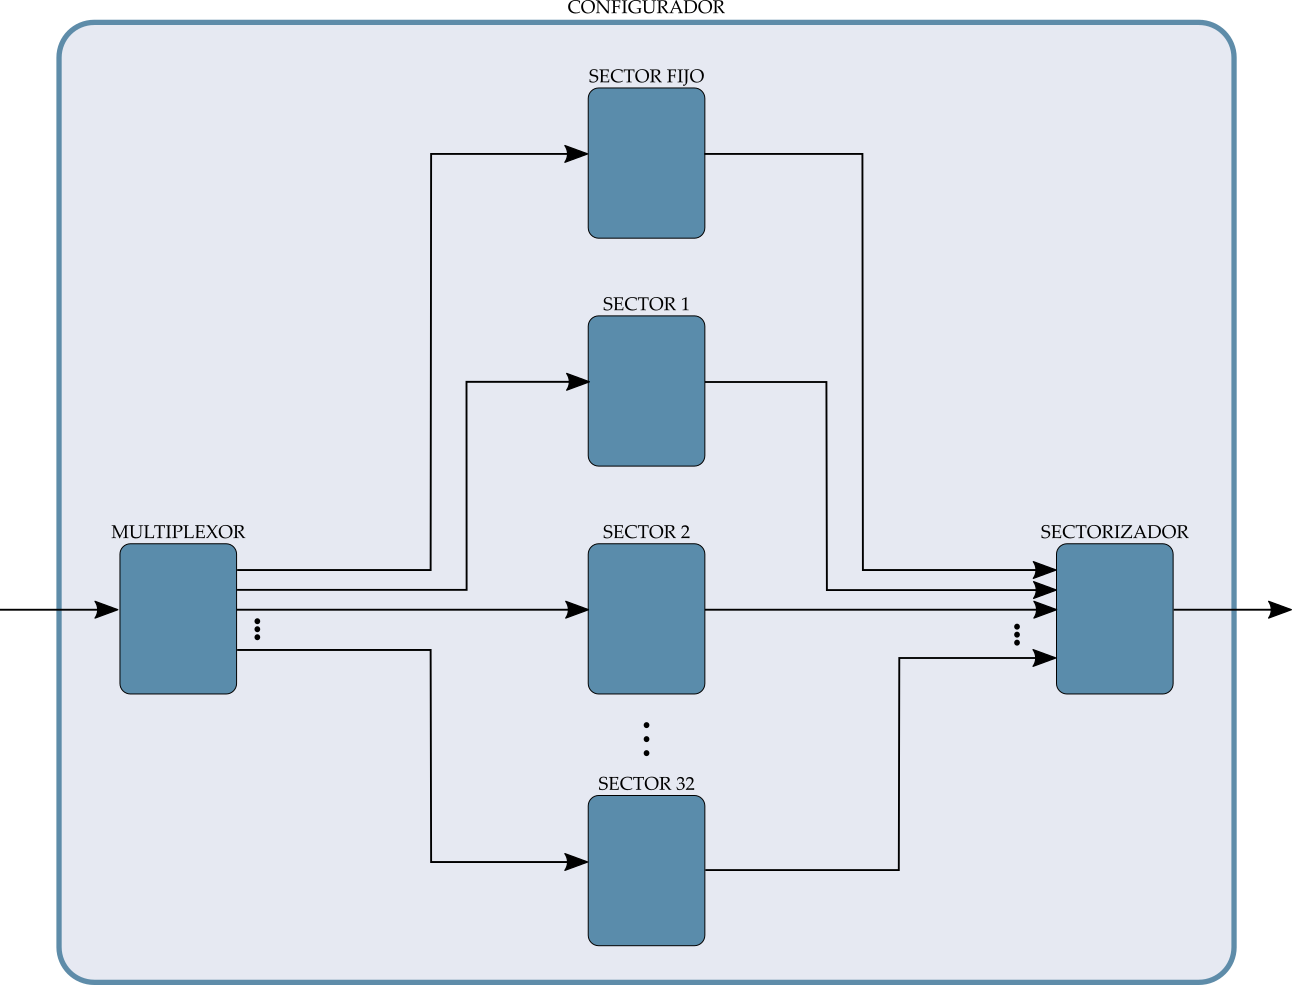
\includegraphics[scale=0.4]{./Figures/configurador_diag_bloques.png}
\caption{Relación entre componentes del Configurador}
\label{diagrama_configurador}
\end{figure}

La relación entre entidades de diseño del configurador y el flujo de información entre estos se ilustra en la figura \ref{diagrama_configurador}. En esta figura multiplexor de entrada no es una entidad de diseño, sino forma parte de la arquitectura del configurador.

Cada componente fue diseñado para realizar las acciones que se describen a continuación.

\subsubsection{Sector fijo}
\begin{itemize}
\item Debe almacenar la configuración existente en sus puertos de entrada cuando se detecte un flanco ascendente de reloj. La salida debe quedar disponible a partir de ese momento.
\end{itemize}

\subsubsection{Registro de entrada}
\begin{itemize}
\item Debe almacenar la configuración existente en sus puertos de entrada cuando se detecte un flanco ascendente de la señal de reloj y este coincida con un nivel alto de la señal correspondiente a la habilitación de carga de configuración. La salida debe quedar disponible a partir de ese momento.
\end{itemize}

\subsubsection{Registro de salida}
\begin{itemize}
\item Debe almacenar la configuración existente en sus puertos de entrada cuando se detecte un flanco ascendente de la señal de reloj y este coincida con un nivel alto de la señal correspondiente al paso por el norte del radar. La salida debe quedar disponible a partir de ese momento.
\end{itemize}

\subsubsection{Sector}
\begin{itemize}
\item Debe poder operar en dos submodos:
	\begin{itemize}
	\item Submodo fijo
	
	
		\begin{itemize}
		\item Debe operar únicamente con los registro de entrada y salida
		\item La carga de configuración en el registro de entrada estará habilitada sí y solo sí el código de sector que se encuentro dentro de la configuración sea igual al código de identificación de ese sector.
		\end{itemize}
	
	
	
	\item Submodo automático
		\begin{itemize}
		\item Debe contar las presencias
		\item En cada paso por el norte debe actualizar el multiplicador almacenado en el registro de salida en función de la cantidad de presencia requerida.
		\item En cada paso por el norte debe resetear los contadores.
		\end{itemize}
	
	
	\end{itemize}
\end{itemize}



\subsubsection{Procesador de presencias}
\begin{itemize}

\item Debe poder configurarse con el submodo en submodo fijo o automático.
\item En submodo fijo debe quedar inactivo con su salida en la decisión correspondiente a "no incrementar".
\item En submodo automático:
	\begin{itemize}
	\item Debe contar las presencias en tres contadores diferentes.
	\item Debe calcular el error absoluto de cada cuenta con la configuración de la cantidad de presencia requerida por el usuario.
	\item Debe decidir si para cada tipo de dato (correspondiente a cada contador) es necesario aumentar o disminuir el multiplicador para la siguiente vuelta.
	\end{itemize}

\end{itemize}

\subsubsection{Ajuste de multiplicador}
\begin{itemize}
\item Debe recibir el valor de decisión proveniente del procesador de presencias.
\item Debe contener una máquina de estados con dos estados, fijo y automático.
\item En modo automático debe modificar el valor del multiplicador almacenado de acuerdo a la decisión del procesador de presencias; puede aumentar o disminuir el valor del multiplicador o no modificarlo.
\item En modo fijo debe quedar inactivo proporcionando a la salida el último multiplicador modificado.
\end{itemize}

\subsubsection{Sectorizador}
\begin{itemize}
\item El grupo de puertos de entrada correspondientes a un sector determinado debe contemplar al menos los datos de selección de tipo de video, multiplicador, algoritmo y coeficiente de ventana.
\item Debe contener tantos grupos de entradas como salidas de configuración de los sectores se utilicen.
\item Debe generar el código de sector actual con las cuentas de rango y azimut.
\item Su salida debe funcionar como un multiplexor cuya llave de selección debe ser el código del sector actual.
\end{itemize}


\subsubsection{Configurador}
\begin{itemize}
\item Debe recibir las cuentas de rango y azimut de los subsistemas encargados de realizar esa cuenta.
\item Debe contar las presencias utilizando tres contadores diferentes.
\item Debe contemplar 2 modos de funcionamiento:
	\begin{itemize}
	\item Modo fijo (o manual): Debe proporcionar a la salida, un valor fijo de multiplicador, algoritmo, tipo de video y ventana deslizante para toda la cobertura.
	\item Modo automático: Debe generar el código de identificación de cada sector predefinido en base a la combinación de los datos de las cuentas de rango y azimut. Debe proporcionar a la salida la configuración almacenada en el sector correspondiente al sector por el que en ese intervalo de tiempo transita el radar.
	\end{itemize}
	
\item Los sectores instanciados deben ser independientes.
\item Debe recibir la configuración del puente HPS y redireccionar la misma al sector correspondiente si el modo de operación es automático o al sector fijo si el modo es fijo.
\item Su salida debe conectarse al CFAR para configurar su forma operación.
\item Debe contar con un multiplexor a la salida que, dependiendo del modo, direccione a los puertos de salida la configuración almacenada en el sector fijo o la que proviene del sectorizador.
\end{itemize}








	